\documentclass{article}
\usepackage[T1]{fontenc}
\usepackage{lmodern}
\usepackage{graphicx}
\usepackage{amsmath,amssymb}
\usepackage[a4paper,margin=2cm]{geometry}
\usepackage[absolute,overlay]{textpos}
\setlength{\TPHorizModule}{1mm}
\setlength{\TPVertModule}{1mm}
\usepackage[indonesian]{babel}
\usepackage{hyperref}
\setlength{\emergencystretch}{2em}
% unit: Halaman 38

\begin{document}

% === Halaman 38 (llm) ===

\section*{How Wiretapping Works}
(sumber: http://www.howstuffworks.com/wiretapping.htm)

\vspace{60mm}

When you open up a phone, you can see that the technology inside is very simple. The simplicity of design makes the phone system vulnerable to surreptitious eavesdropping.

\vspace{10mm}

Inside a standard phone cord, you'll find a red wire and a green wire. These wires form a circuit like the one you might find in a flashlight. Just as in a flashlight, there is a negatively-charged end and a positively-charged end to the circuit. In a telephone cord, the green wire connects to the positive end and the red cord connects to the negative end.

% deskripsi: Foto bagian dalam telepon genggam lama yang memperlihatkan kabel-kabel sederhana.
% bbox normalisasi: [0.1170, 0.2370, 0.4850, 0.7320]
\begin{textblock*}{77.28mm}(24.57mm,70.39mm)
\noindent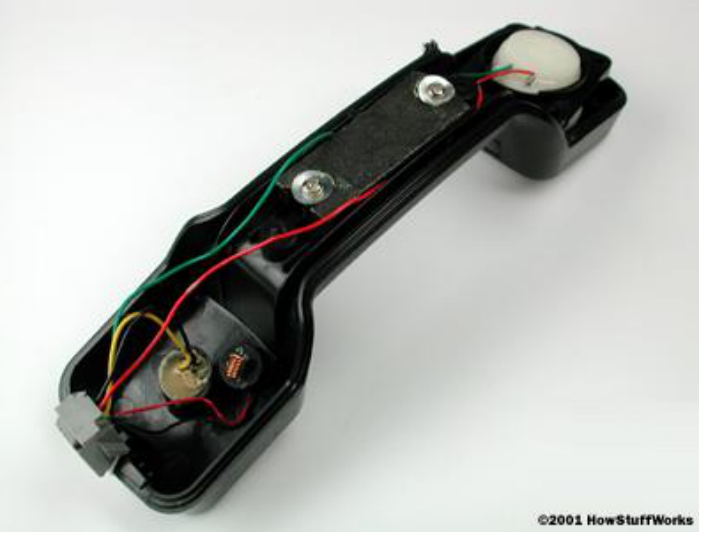
\includegraphics[width=77.28mm,height=147.01mm]{../../images/llm/page_038_img_01.png}%
\end{textblock*}

% deskripsi: Foto kabel telepon yang dikupas ujungnya, memperlihatkan kabel merah dan hijau.
% bbox normalisasi: [0.5140, 0.2370, 0.9230, 0.6540]
\begin{textblock*}{85.89mm}(107.94mm,70.39mm)
\noindent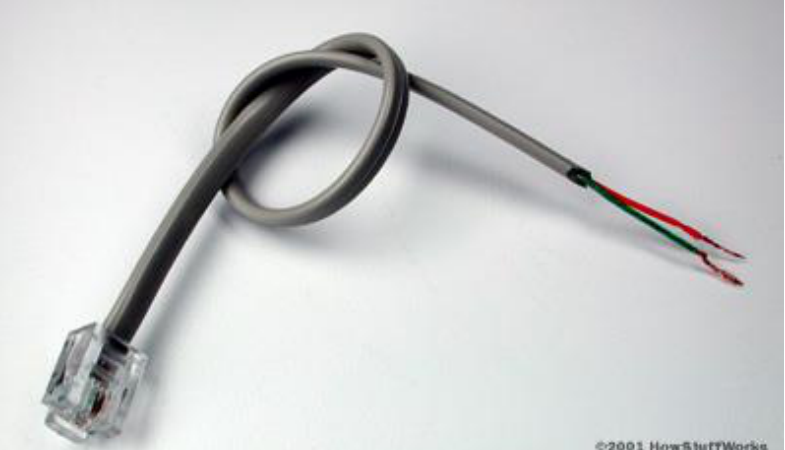
\includegraphics[width=85.89mm,height=123.85mm]{../../images/llm/page_038_img_02.png}%
\end{textblock*}

\end{document}
